% Created 2020-07-08 mié 11:52
% Intended LaTeX compiler: pdflatex
\documentclass[presentation,aspectratio=1610]{beamer}
\usepackage[utf8]{inputenc}
\usepackage[T1]{fontenc}
\usepackage{graphicx}
\usepackage{grffile}
\usepackage{longtable}
\usepackage{wrapfig}
\usepackage{rotating}
\usepackage[normalem]{ulem}
\usepackage{amsmath}
\usepackage{textcomp}
\usepackage{amssymb}
\usepackage{capt-of}
\usepackage{hyperref}
\usepackage{khpreamble}
\usepackage{amssymb}
\DeclareMathOperator{\shift}{q}
\DeclareMathOperator{\diff}{p}
\usetheme{default}
\author{Kjartan Halvorsen}
\date{2020-07-09}
\title{Control Computarizado - PID digital}
\hypersetup{
 pdfauthor={Kjartan Halvorsen},
 pdftitle={Control Computarizado - PID digital},
 pdfkeywords={},
 pdfsubject={},
 pdfcreator={Emacs 26.3 (Org mode 9.3.6)}, 
 pdflang={English}}
\begin{document}

\maketitle


\section{Discretization - repetición}
\label{sec:orgebce0ad}
\begin{frame}[label={sec:orgb28288d}]{Discretización de un controlador continuo}
\begin{center}
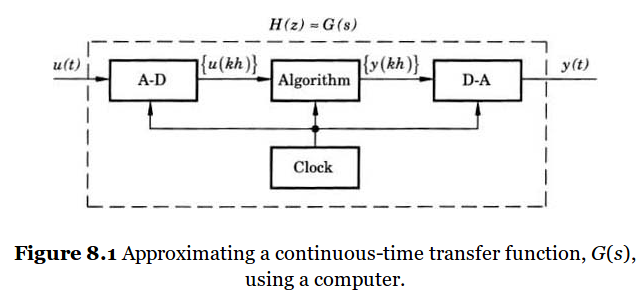
\includegraphics[width=0.7\linewidth]{../../figures/fig8-1.png}
\end{center}

\begin{itemize}
\item Dado un controlador obtenido de un diseño en tiempo continuo
\item Es necesario discretizarlo para implementar en una computadora
\end{itemize}
\end{frame}

\begin{frame}[label={sec:org0efb46c}]{Métodos de discretización}
Introduciendo el operador diferencial:  \(\diff f(t) = \frac{d}{dt} f\)

\begin{enumerate}
\item Euler (diferencia hacia adelante) \(\diff \approx \frac{\shift -1}{h}\). Substituir
\[ s = \frac{z-1}{h} \] en \(F(s)\) para obtener
\[ F_d(z) = F(s')|_{s'=\frac{z-1}{h}}. \]
\item Euler hacia atras \(\diff \approx \frac{1 - \shift^{-1}}{h} = \frac{\shift -1}{h\shift}\). Substituir
\[ s = \frac{z-1}{zh} \] en \(F(s)\) para obtener
\[ F_d(z) = F(s')|_{s'=\frac{z-1}{zh}}. \]
\end{enumerate}
\end{frame}

\begin{frame}[label={sec:orgff9ce2f}]{Métodos de discretización}
\begin{enumerate}
\setcounter{enumi}{2}
\item El método de Tustin (transformada bilineal). Substituir
\[ s = \frac{2}{h}\frac{z-1}{z+1} \] en \(F(s)\) para obtener
\[ F_d(z) = F(s')|_{s'=\frac{2}{h}\cdot \frac{z-1}{z+1}}. \]
\item Discretización invariante a la rampa. Similar a discretización con ROC. La transformada z de una rampa es  \(\frac{zh}{(z-1)^2}\) y su transformada de Laplace \(1/s^2\). La discretización es dado por
\[ F_d(z) = \frac{(z-1)^2}{zh} \ztrf{\laplaceinv{\frac{F(s)}{s^2}}}. \]
\end{enumerate}
\end{frame}

\begin{frame}[label={sec:org8c29b43}]{Mapeo de la región estable del plano \(s\)}
\begin{center}
 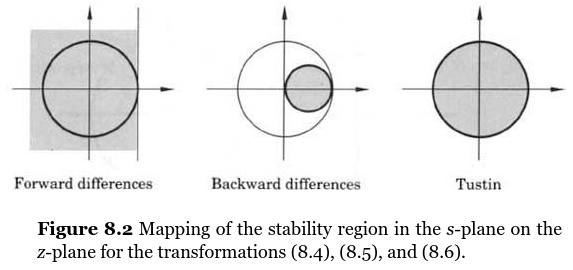
\includegraphics[width=0.79\linewidth]{../../figures/fig8-2.png}\\
{\tiny Åström and Wittenmark \emph{Computer-controlled systems}}
\end{center}
\end{frame}

\section{PID}
\label{sec:orgb269cd2}
\begin{frame}[label={sec:org974df95}]{PID tipo ISA}
ISA - International Society of Automation

\[ F(s) = K\left( 1 + \frac{1}{T_i s} + T_d s\right) \]

Con filtro pasobajo para el parte derivativo

\[ F(s) = K\left( 1 + \frac{1}{T_i s} + \frac{T_d s}{\frac{T_d}{N} s + 1}\right), \quad N \approx 3\; - \; 10 \]
\end{frame}

\begin{frame}[label={sec:org8a73c62}]{PID tipo ISA - ejercicio}
\[ F(s) = K\left( 1 + \frac{1}{T_i s} + \frac{T_d s}{\frac{T_d}{N} s + 1}\right), \quad N \approx 3\; - \; 10 \]

\alert{Actividad en pares} Dibuja el diagrama de Bode (solo la magntitúd)  del parte derivativo \[F_d(s) = \frac{T_d s}{\frac{T_d}{N} s + 1}\] usando las approximaciones de baja y alta frecuencia
\begin{align*}
 \text{$\omega$ small:} \quad & F_d(i\omega) \approx T_d i\omega \\
 \text{$\omega$ large:} \quad & F_d(i\omega) \approx \frac{T_d i \omega }{\frac{T_d}{N} i\omega} = N
\end{align*}
\end{frame}

\begin{frame}[label={sec:org2540245}]{PID tipo ISA - solución}
\[ F(s) = K\left( 1 + \frac{1}{T_i s} + \frac{T_d s}{\frac{T_d}{N} s + 1}\right), \quad N \approx 3\; - \; 10 \]

\begin{center}
  \def\Td{1}
  \def\NN{6}
  \begin{tikzpicture}
    \begin{loglogaxis}[
    clip=false,
    width=14cm,
    height=5cm,
    ylabel={$|F_d(i\omega)|$},
    xlabel={$\omega$},
    ytick={\NN},
    yticklabels={$N$},
    xtick = {0.01, 0.1, 1, 10, 100}, 
    xticklabels={$\frac{0.01}{T_d}$, $\frac{0.1}{T_d}$, $\frac{1}{T_d}$, $\frac{10}{T_d}$, $\frac{100}{T_d}$},
    ]
      \addplot[red!80!black, no marks, domain=0.01:100, samples=20] {\Td*x/sqrt(1 + pow(\Td/\NN * x, 2))};
      \draw[orange, dashed] (axis cs: \NN/\Td, \NN) -- (axis cs: \NN/\Td, 0.003) node[below] {$\frac{N}{Td}$};
    \end{loglogaxis}

 \end{tikzpicture}
\end{center}
\end{frame}
\end{document}